\section{The motion of Charged Particles in Magnetic Fields}
When a charged particle go through a magnetic field, we can seperate the motion in to two components. 
\begin{center}
    \tikzset{every picture/.style={line width=0.75pt}} %set default line width to 0.75pt        

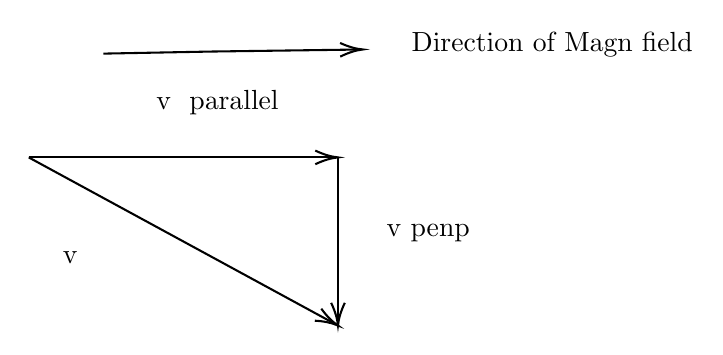
\begin{tikzpicture}[x=0.75pt,y=0.75pt,yscale=-1,xscale=1]
%uncomment if require: \path (0,300); %set diagram left start at 0, and has height of 300

%Straight Lines [id:da42319733275995863] 
\draw    (252,126) -- (399,126) ;
\draw [shift={(401,126)}, rotate = 180] [color={rgb, 255:red, 0; green, 0; blue, 0 }  ][line width=0.75]    (10.93,-3.29) .. controls (6.95,-1.4) and (3.31,-0.3) .. (0,0) .. controls (3.31,0.3) and (6.95,1.4) .. (10.93,3.29)   ;
%Straight Lines [id:da8555331334957245] 
\draw    (401,126) -- (401,205) ;
\draw [shift={(401,207)}, rotate = 270] [color={rgb, 255:red, 0; green, 0; blue, 0 }  ][line width=0.75]    (10.93,-3.29) .. controls (6.95,-1.4) and (3.31,-0.3) .. (0,0) .. controls (3.31,0.3) and (6.95,1.4) .. (10.93,3.29)   ;
%Straight Lines [id:da8190606414124877] 
\draw    (252,126) -- (399.24,206.04) ;
\draw [shift={(401,207)}, rotate = 208.53] [color={rgb, 255:red, 0; green, 0; blue, 0 }  ][line width=0.75]    (10.93,-3.29) .. controls (6.95,-1.4) and (3.31,-0.3) .. (0,0) .. controls (3.31,0.3) and (6.95,1.4) .. (10.93,3.29)   ;
%Straight Lines [id:da9159826287918194] 
\draw    (288,76) -- (340,75) -- (411,74.03) ;
\draw [shift={(413,74)}, rotate = 179.22] [color={rgb, 255:red, 0; green, 0; blue, 0 }  ][line width=0.75]    (10.93,-3.29) .. controls (6.95,-1.4) and (3.31,-0.3) .. (0,0) .. controls (3.31,0.3) and (6.95,1.4) .. (10.93,3.29)   ;

% Text Node
\draw (423,157) node [anchor=north west][inner sep=0.75pt]   [align=left] {v penp};
% Text Node
\draw (312,92) node [anchor=north west][inner sep=0.75pt]   [align=left] {v \ parallel};
% Text Node
\draw (267,170) node [anchor=north west][inner sep=0.75pt]   [align=left] {v};
% Text Node
\draw (435,64) node [anchor=north west][inner sep=0.75pt]   [align=left] {Direction of Magn field};


\end{tikzpicture}
\end{center}



\subsubsection{What will the motion of the particle look like}
\begin{itemize}
    \item If the magnetic field is large and uniform, $\vec{v_{\parallel}}$ will remain constant
    \item Because the magnetic force is always perpendicular to $\vec{v_{\perp}}$, it will not affect the magnitude of $\vec{v_{\perp}}$, 
    it will only cause the direction to change. 
    \item If the magnetic field doesn't change, the $F_M$ will be constant
    \item Thus, we get a \underline{corkscrew} motion. 
\end{itemize}

\begin{figure}[!h]
    \centering
    \includegraphics[width=0.3\textwidth]{pictures/4.8.1.png}
    \caption{Motion of che charged particle}
\end{figure}

\subsubsection{Aurora Borealis}
The sun emits charged particles (ions), we call this the solar wind. When the solar wind reaches the Earth, the charged particles can become trapped 
in the Earth's mag field. 

\begin{figure}[!h]
    \centering
    \includegraphics[width=0.3\textwidth]{pictures/4.8.2.png}
    \caption{Aurora Borealis}
\end{figure}

The ions flow the mag field towards one of the poles. The ions start to descend as they get closer to the poles (to regions where the air is more dense). 
When one of the ions collide with an air particle (either oxygen or nitrogen) light is given off. If enough collisions occur, we are able to see the light. 

\subsubsection{Mass Spectrometers}
Under the right conditions a particle that enters a magnetic field will undergo full \underline{uniform circular motion}\\

Following two conditions must be met:
\begin{itemize}
    \item The magnetic field must be relatively large and uniform. 
    \item The particle must be travelling penpendicular. 
\end{itemize}

\textbf{Procedures}\\

Mass spectrometer can be used to determine the mass of a particle with following steps:
\begin{itemize}
    \item Something to inject particles into the spectrometer, at the correct plate of a particle. 
    \item Something that causes the particles to become ionized
    \item A particle accelerator to "shoot" the particles into a magnetic field
    \item A large, uniform magnetic field
    \item A moveable ion detector (Used to determine where the ion emerges from the magnetic field)
\end{itemize}

\begin{theorem}
    If we can determine the $q$ of the particle; Magnetic Field Strength ($B$); Potential Difference $\Delta v$ and radius of the particle's circular motion, 
    the mass of the particle can be calculated using this formula:
    \begin{equation*}
        m = \frac{
            \left|q\right| B^2 R^2
        }{
            2 \left|\Delta v\right|
        }
    \end{equation*}
    Please do not include the sign when you are using the formula. 
\end{theorem}

Here is another formula that maybe useful:
\begin{gather*}
    \Delta \vec{F} = m\vec{a}\\
    F_M = ma_c\\
    \left|q\right|vB\sin\theta = m\frac{v^2}{R}
\end{gather*}